\chapter{Nouvelle architecture de la grille horaire de \diamant{}} 

Ce chapitre pr�sente la nouvelle grille horaire, d�crit les interpr�tations et l'�num�ration des diff�rentes
informations requises par \diamant{}.

\section{pr�sentation de la grille horaire}

Cette nouvelle grille horaire sera stock�e dans un fichier XML comme repr�sent� � la figure \ref{xmltt} et elle permettra de traiter ind�pendamment chaque cycle.

\subsection{Exemple des donn�es qu'elle contient}

\begin{figure}[h]
  % Requires \usepackage{graphicx}
  \begin{center}
    \includegraphics[width=250pt]{Images/TTxmlContains.eps}
    \caption{Fichier XML de la grille horaire}\label{xmlcontains}
  \end{center}
\end{figure}

\subsection{Signification des donn�es}

Le fichier XML contenant les informations sur la grille horaire est organis� de mani�re hi�rarchique (arbre). Chaque information est encapsul�e dans un \emph{tag}. Chaque \emph{tag} donne le grade hi�rarchique de l'information sur l'arbre. Cette hi�rarchie est d�crite comme suit:
\begin{itemize}
    \item le tag \emph{DXTimeTable}:
    \item le tag \emph{TTweek}:
    \item le tag \emph{TTdays}:
    \item le tag \emph{TTday}:
    \item le tag \emph{TTsequences}:
    \item le tag \emph{TTsequence}:
    \item le tag \emph{TTperiods}:
    \item le tag \emph{TTperiod}:
\end{itemize}    


\begin{figure}[h]
  % Requires \usepackage{graphicx}
  \begin{center}
    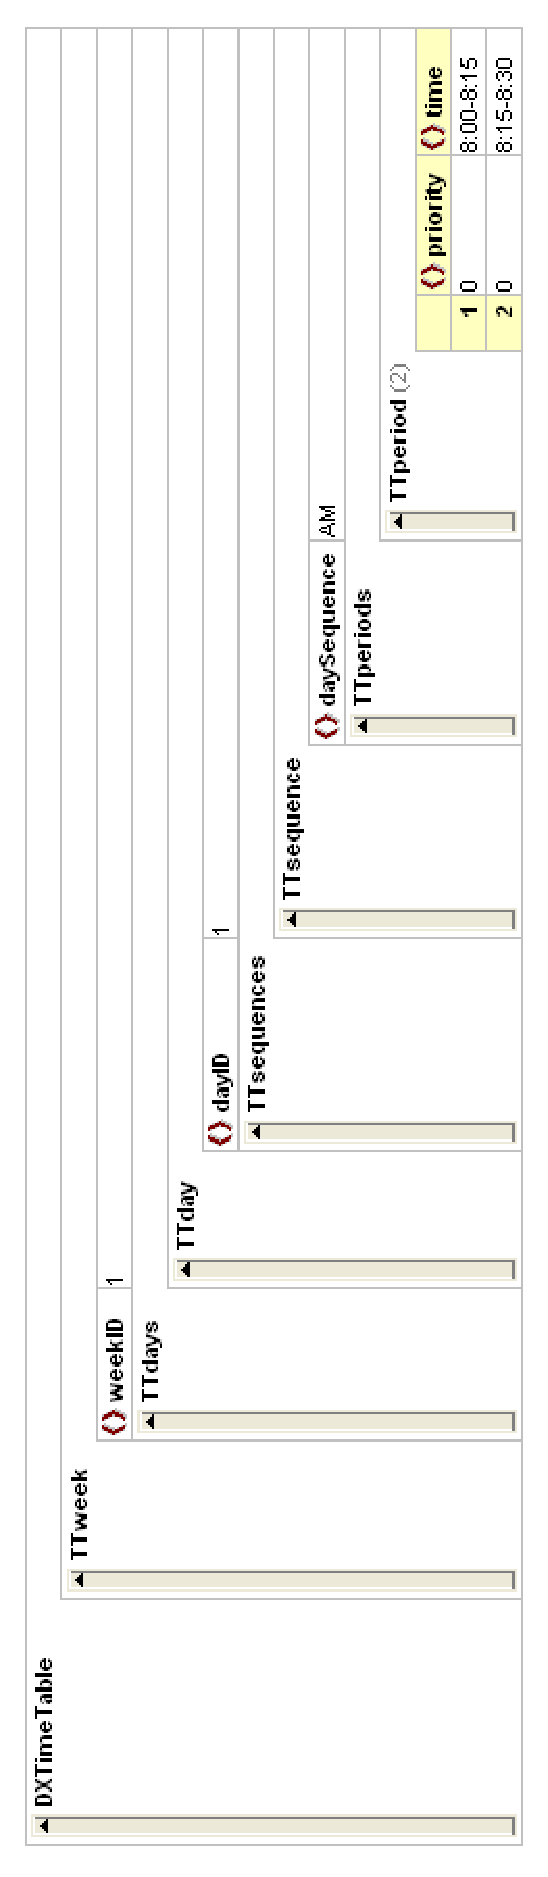
\includegraphics[width=200pt]{Images/TTxmlModel.eps}
    \caption{Schema de la grille horaire}\label{xmltt}
  \end{center}
\end{figure}

\section{Avantages et limites de cette architecture}
